%-------------------------------------------------------------------------------
\section{Introduction}
\label{s:intro}
%-------------------------------------------------------------------------------

Cloud providers like AWS and Google, as well as deployment management systems
like Kubernetes, allow users to run services by attaching to each an amount of
resources the service will get. This includes compute (a number of vCPUs),
memory, and sometimes network bandwidth~\cite{aws-ec2-resources,
kubernetes-resources}; the resource this work focuses on is CPU. The guarantee
developers get is that the service will have undisturbed access to that amount
of resources.

Enforcing this guanatee is hard. If providers leave the CPUs idle so they are
available when the service needs them, that leads to a utilization problem. The
load on most applications run in the cloud is variable and unpredictable, so to
account for this developers choose the amount of resources to reserve based on
the expected peak load~\cite{borg, nu, overprovision}. This means that services
with reserved resources rarely use the full reservation they asked for. 

What most systems do instead is allow other workloads to run opportunistically
on temporarly unutilized resources. This includes so-called \textit{best effort}
workloads, which have no reservations, as well letting services with
reservations temporarily \textit{burst}, meaning use more CPUs than they asked
for. This solves the utilization problem, without requiring compromises on the
guarantees made: services with reservations get access to the CPUs they
requested when desired, while best effort or bursting services can make use of
otherwise idle resources.

Kubernetes follows presicely this model. Services fall into three quality of
service (QOS) classes: \textit{Guaranteed}, which have requests (\ie{}
reservations) as well as limits, \textit{Burstable}, which have requests and no
limits, and \textit{Best Effort}, which have
neither~\cite{kubernetes-pod-qos-types}. Guaranteed services are the last to be
evicted from a node experiencing high load, and give more predictable
performance, whereas the Burstable class allows applications with bursty load to
opportunistically make use of available resources, thereby better utilizing the
resources Kubernetes is running on.

AWS similarly supports both guaranteed- and burstable-style reservations, with
their M and T instance types~\cite{aws-ec2-burstable,aws-ec2-resources}. In this
case the motivation for customers to use the burstable-style instance rather
than overprovisioning on guaranteed-style is pricing.


\begin{figure}[t]
    \centering
    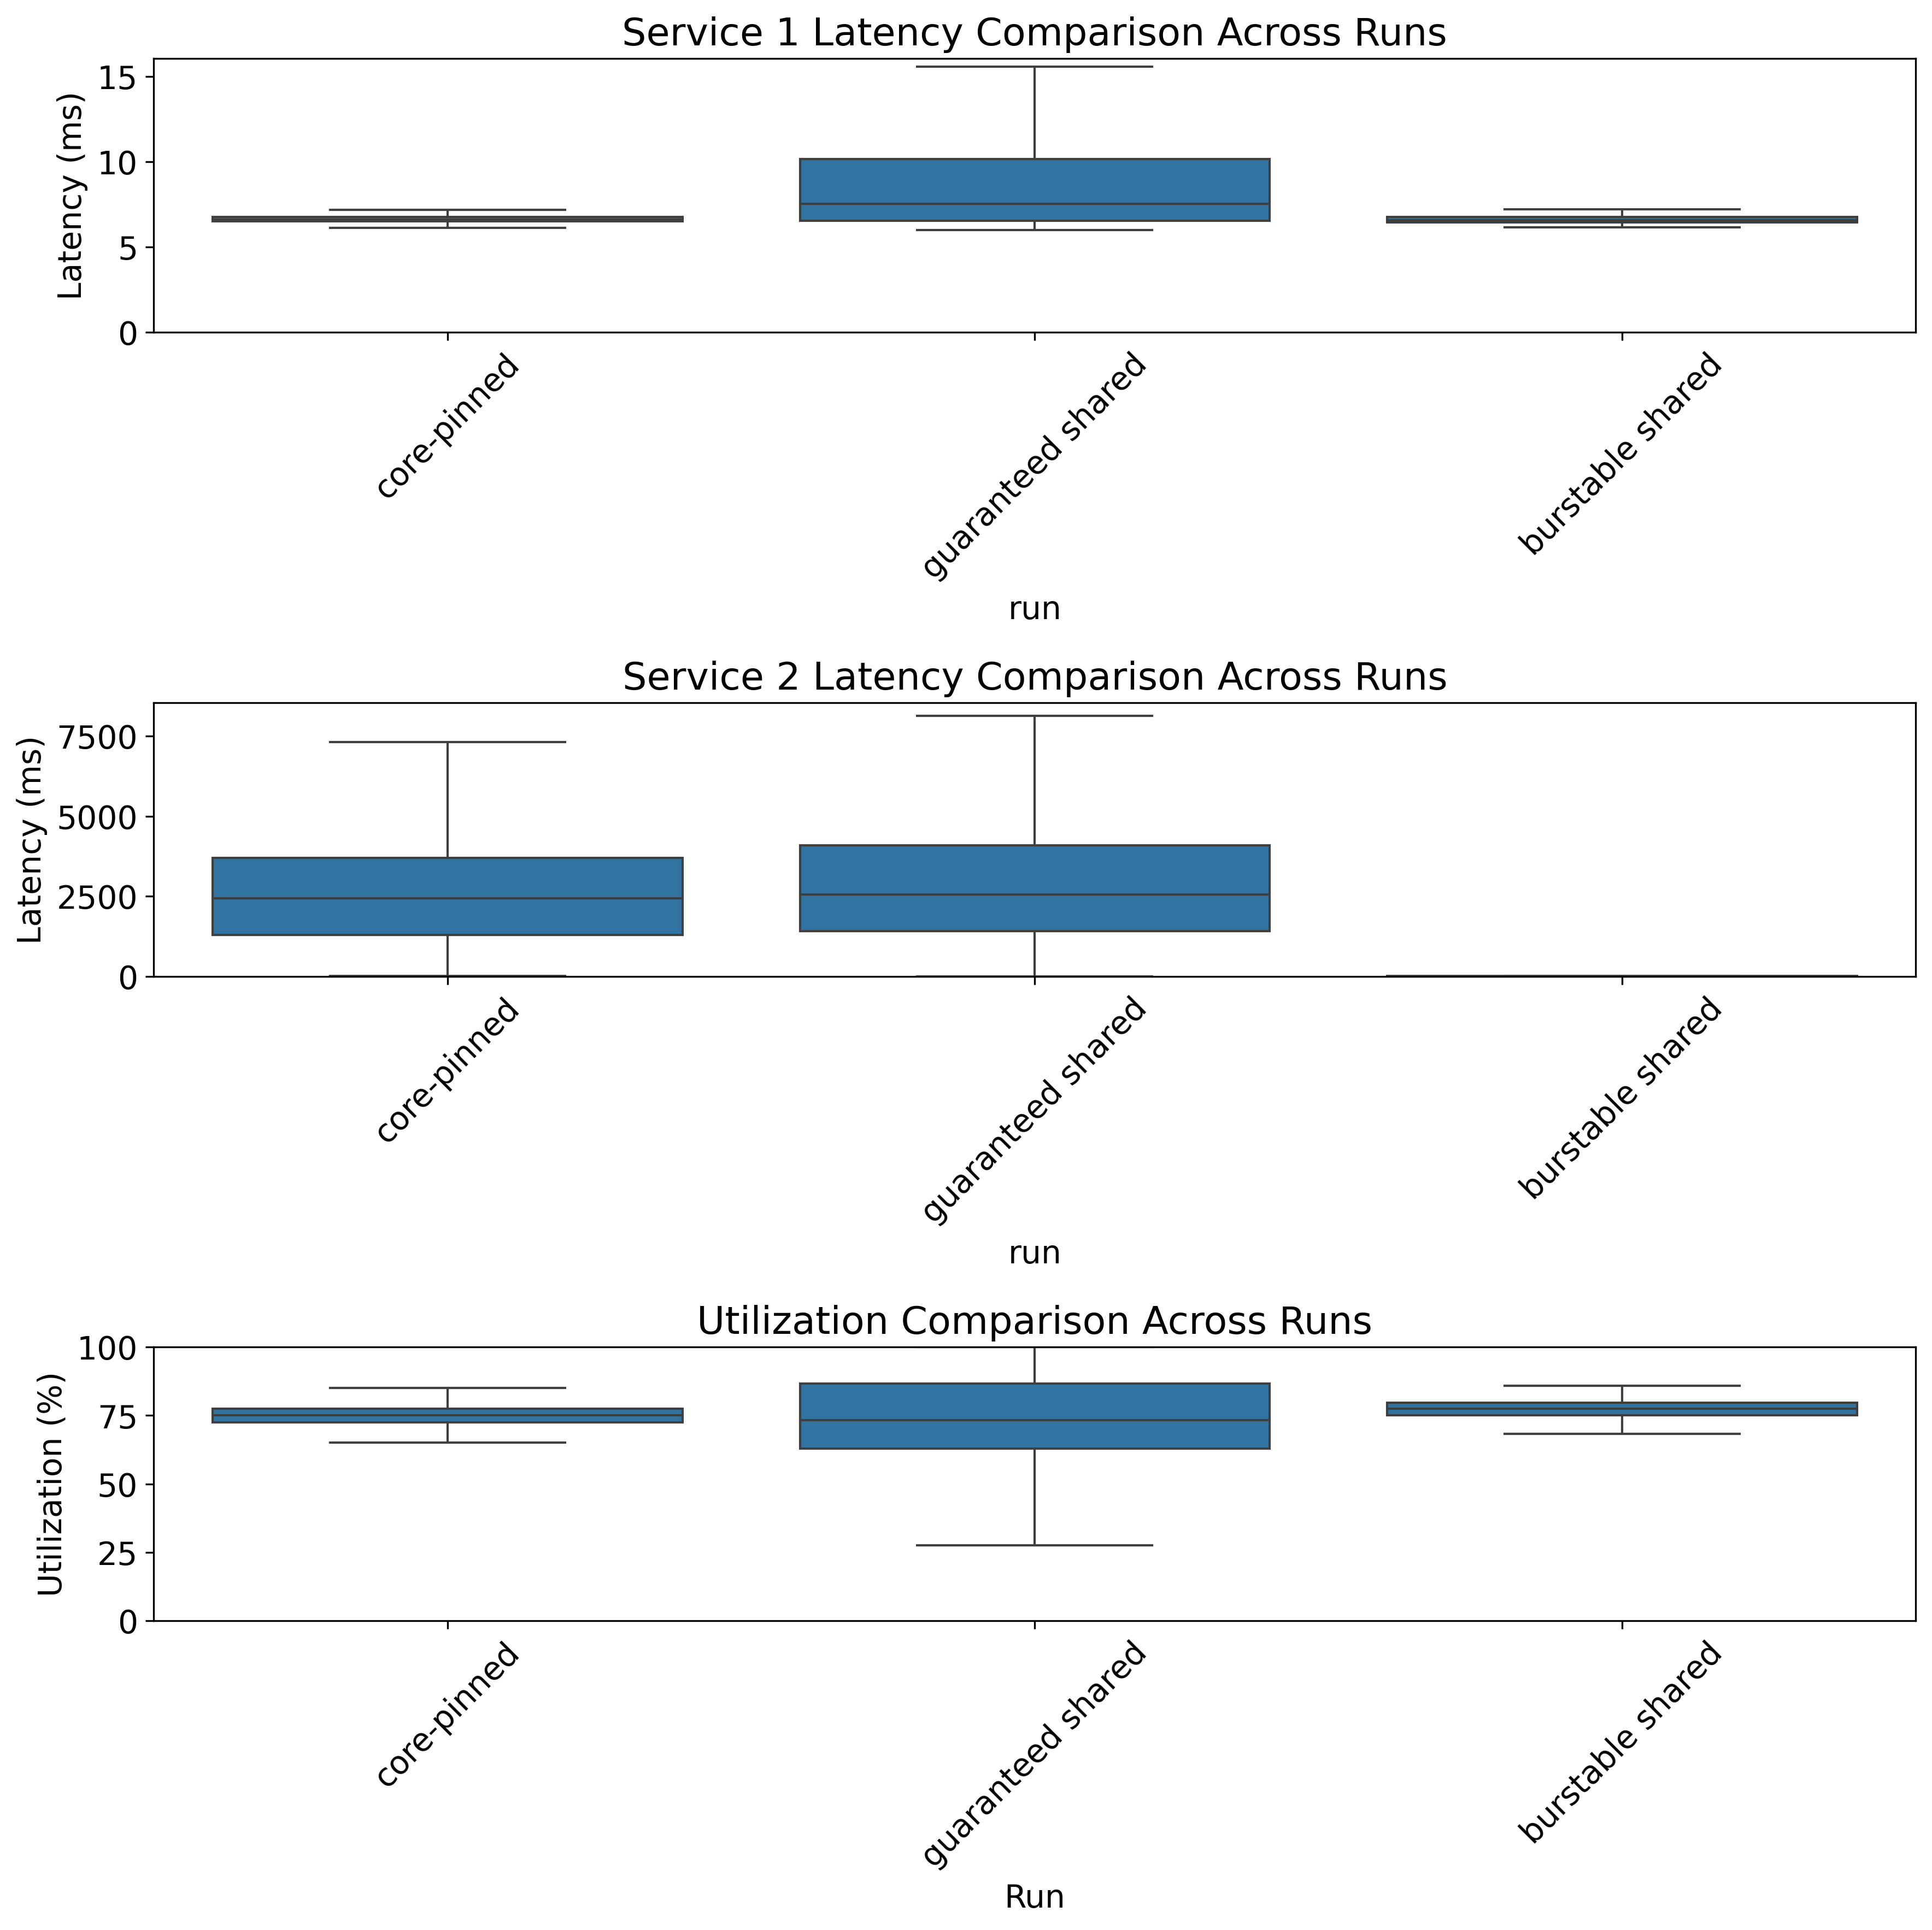
\includegraphics[width=\columnwidth]{graphs/kubernetes-lc-lc-cmp.png}
    \caption{In Kubernetes, running anything alongside a server in the
    Guaranteed QOS class affects the server's
    performance}\label{fig:kubernetes-qos-cmp}
\end{figure}

\begin{figure}[t]
    \centering
    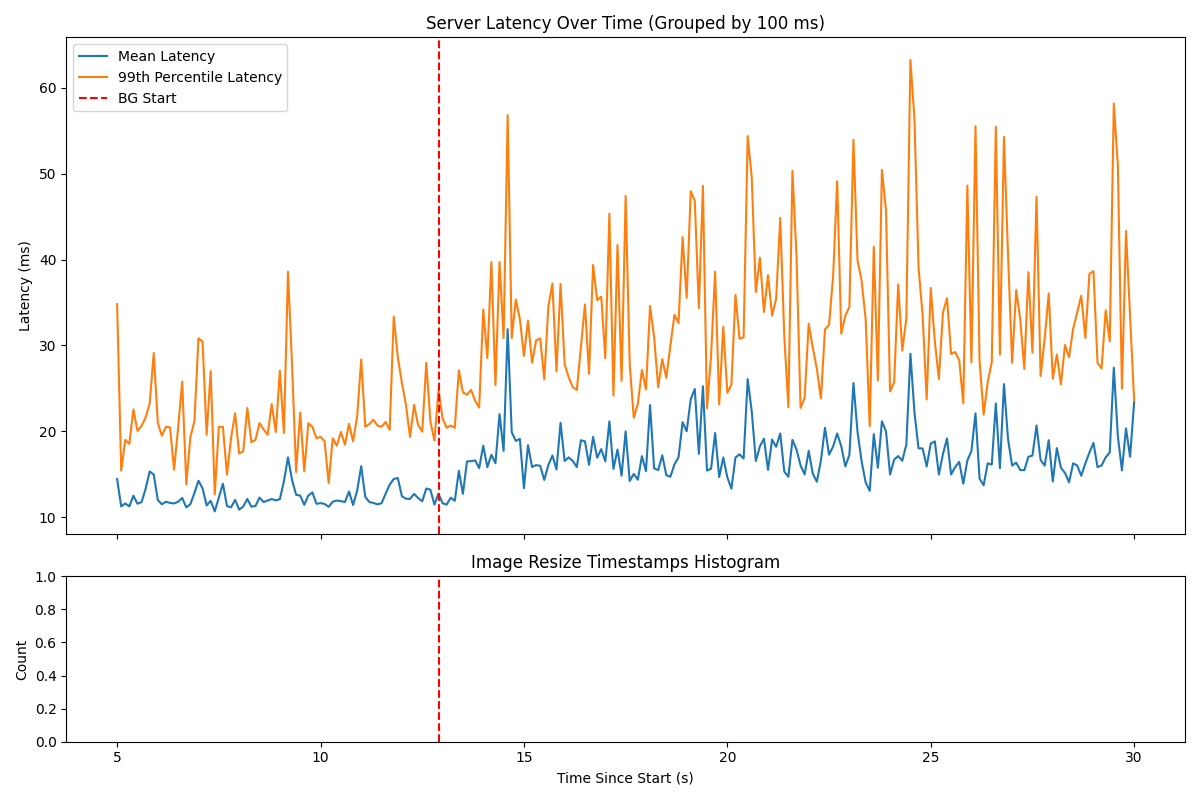
\includegraphics[width=\columnwidth]{graphs/kubernetes-unedited.png}
    \caption{Running a BestEffort affects the server's
    performance}\label{fig:kubernetes-unedited}
\end{figure}

We find that current popular scheduling systems fail to properly enforce
reservations. We use as a case study a small but realistic social network web
application, which we run using Kubernetes. We run alongside it different other
classes: in one experiment, we run another server in either the Guaranteed and
Burstable class, and in another we run a best effort workload alongside the
server. 

In \autoref{fig:kubernetes-qos-cmp} we show the results of the first experiment.
We run two servers, and compare the performance in three settings: both are
pinned to their own cores, both running in the Guaranteed class, and the web
server running in the Guaranteed class but the other in the Burstable class. The
graphs show the utilization and performance benefit of using the Burstable
class, but also show that running either class alongside the web server affected
its end-to-end latencies.

\autoref{fig:kubernetes-unedited} shows the result of running a best effort
workload, using the BestEffort class, alongside the web server. The top graph of
plots the end-to-end latency of an endpoint that gets a users feed and applies a
moderation; the bottom graph shows the throughput of a best effort image resize
job. After the image resize job starts running, the mean response latency of the
web application jumps from $\sim$7ms to $\sim$15ms, and the 99th percentile
latency from $\sim$10ms to $\sim$25ms.

\hmng{edited up to here}

Understanding why Kubernetes fails to honor the web application's reservation
requires looking at the underlying mechanism enforcing the CPU reservation:
Linux's \cgroups{}. In fact, most modern containers rely on \cgroups{} for CPU
isolation: all Open Container Initiative (OCI) compliant containers, including
Kubernetes but also Docker, CRI-O, and containerd
do~\cite{oci-cgroups,docker-docs-cgroups,container-isolation-article}. VM
frameworks, including Firecracker, AFaas and libvirt, also rely on \cgroups{} to
manage CPU time reservation~\cite{firecracker-cgroups,afaas,libvirt-cgroups}.

Weight is the part of the \cgroups{} interface these systems use for enforcing
the reservations LC applications have, while still allowing BEs without
reservations to run opportunistically.\footnote{Other operating systems expose a
similar interface, for instance Windows exposes a number of shares.} Kubernetes
creates one top level group for all best effort services, called
\texttt{kubepods-besteffort}, inside which all BE pods are placed, and assigns
it the lowest possible weight of 1. Pods with reservations are separated into
Burstable and Guaranteed, the main difference being that Guaranteed pods require
a limit to be set on the resources it can use. Kubernetes calculates the weight
that each pod gets based on the amount of milliCPUs it requests. For instance,
in the \autoref{fig:kubernetes-unedited} experiment, the web application service
ran in the Guaranteed class and asked for 4 CPUs, and Kubernetes assigned the
underlying pod a weight of 157.

The \cgroups{} documentation specifies that each group should get CPU time
proportional to its weight as a share of the sum of weights of runnable
groups~\cite{cgroups-kerneldocs}. However, the latency increase we see after
starting the best effort tasks in \autoref{fig:kubernetes-unedited} is much more
than the 1\% CPU time the server should be losing out on based on its weight. As
we show in more detail in \autoref{s:problem}, the problem that leads to the
increased latencies observed is that Linux will run a low weight process on one
core, unaware that a high weight process is runnable and waiting on another.
This happens because Linux uses per-CPU runqueues, which avoids the overheads of
having a global runqueue. A key challenge this work addresses is managing this
tension between how often the scheduler has to look at all the other cores'
runqueues to enforce reserved processes' priority globally, while still running
best effort ones opportunistically.

Our approach addresses this challenge by creating a new priority class for best
effort tasks to run in, \beclass{}, and enforcing it in the scheduler via
priority scheduling. Linux already has other classes between which it enforces
strict priority, which are designed and used for real time applications
(\autoref{ss:approach:linux-classes-isolate}); the proposed \beclass{} sits
below the default scheduling class. As we show in
\autoref{ss:approach:solves-problems}, putting best effort processes in a
separate class from those with reservations makes it viable to enforce those
reservations across cores, because it reduces the number of times the scheduler
is required to look at all the other cores' runqueues. Enforcing weights across
cores requires the scheduler to do so every scheduling tick, but with a separate
class it only has to look at other cores on \textit{class boundary crossings}:
every time a core switches from running an LC process to running a BE on, and
every time it enqueues an LC process.

A challenge with creating a separate priority class arises when the LC class is
under high load: completely starving best effort processes can lead to issues
such as deadlocks, broken TCP connections, or missed timers. The goal is to make
the priority of processes with reservations over those without as strict as
possible, while still allowing BE processes to resume execution normally once
the load goes down, even if the high load lasts for multiple minutes.

We address this challenge by enabling best effort processes to exist in an
ephemeral state called \textit{parked}, which they enter when the CPU
utilization is high enough that processes with a reservation account for all the
CPU time. While load remains high, the scheduler ensures that the parked BE's
user-space process doesn't run and consume resources, but continues to run the
kernel-space handlers that manage critical state, including TCP connections and
timers, on behalf of the BE processes. 

We implement \beclass{} in Linux on top of an existing scheduling policy called
\schedidle{}, and show that it is able to significiantly improve Linux's ability
to honor reservations while sharing CPUs with best effort workloads: in the same
Kubernetes experiment, the increase in average latency when starting a BE
workload goes from $>$2x to 0. The contributions of this paper are thus as
follows: 
\begin{enumerate}
    \item identifying as the reason LC tasks' reservations are often violated is
    that \cgroups{} does a poor job of enforcing the weights across cores;
    \item the design of \beclass{}, a new class for best effort tasks whose goal
    is to enforce reservations in the presence of BE processes by using priority
    scheduling, that reduces the points in time it needs to look at other core's
    runqueues, as well as enforcing the parked state
    \item an implementation of \beclass{} in Linux
\end{enumerate}
